\documentclass[a4paper]{article}

\usepackage{array}
\usepackage[
    style=numeric, 
    backend=biber, 
    sorting=none
]{biblatex}
\usepackage{graphicx}
\usepackage{enumitem}
\usepackage{geometry}
\usepackage{sectsty}
\usepackage{indentfirst}
\usepackage{times}
\usepackage{listings}
\usepackage{longtable}

\setlist{
  listparindent=\parindent,
  parsep=0pt,
}

% code block style
% -- Defining colors:
\usepackage[dvipsnames]{xcolor}
\definecolor{codegreen}{rgb}{0,0.6,0}
\definecolor{codegray}{rgb}{0.5,0.5,0.5}
\definecolor{codepurple}{rgb}{0.58,0,0.82}
\definecolor{backcolour}{rgb}{0.95,0.95,0.92}% Definig a custom style:
\lstdefinestyle{mystyle}{
    backgroundcolor=\color{backcolour},   
    commentstyle=\color{codepurple},
    keywordstyle=\color{NavyBlue},
    numberstyle=\tiny\color{codegray},
    stringstyle=\color{codepurple},
    basicstyle=\ttfamily\footnotesize\bfseries,
    breakatwhitespace=false,         
    breaklines=true,                 
    captionpos=t,                    
    keepspaces=true,                 
    numbers=left,                    
    numbersep=5pt,                  
    showspaces=false,                
    showstringspaces=false,
    showtabs=false,                  
    tabsize=2
}% -- Setting up the custom style:
\lstset{style=mystyle}

\sectionfont{\centering}
\addbibresource{citation.bib}
\graphicspath{{./images/}}
\geometry{a4paper, top=4.0cm, bottom=3.0cm,
          left=4.0cm, includehead, includefoot}
\renewcommand\contentsname{Daftar Pustaka}
\emergencystretch=2em

% bab command
\newcommand{\bab}[2]{\setcounter{section}{#1}\addtocounter{section}{-1}\section{Bab #1. #2}}

\begin{document}
\linespread{1.5}

\title{Marketplace For Hobby}
\author{Aldih Suhandi, Chandra Wijaya, Ibrahim Seto Aditama}

\maketitle
\begin{figure}[h]
    \centering
    
\includegraphics[width=10cm]{logo_binus.png}\\
    Binus University\\
    2022
\end{figure}
\begin{figure}[h]
    \centering
    Diperiksa Oleh**\\
    \vspace{15mm}
    \begin{tabular}{@{}p{2.5in}@{}}
    \centering
    Nama Dosen - Kode Dosen
    \end{tabular}
\end{figure}

\newpage
\addcontentsline{toc}{section}{\protect\numberline{}Daftar Pustaka}
\tableofcontents

\newpage
\section*{Bab 1. Pendahuluan}
\addcontentsline{toc}{section}{\protect\numberline{}Bab 1. Pendahuluan}

\subsection*{1.1 Latar Belakang}
\addcontentsline{toc}{subsection}{\protect\numberline{}1.1 Latar Belakang}

Perkembangan teknologi yang pesat telah melahirkan banyak teknologi baru yang dapat membantu dan mempermudah kita sebagai manusia dalam menjalankan kehidupan dan melaksanakan tugas dan keinginan kita. Dari perkembangan teknologi tersebut yang memiliki dampak yang cukup tinggi adalah internet, yang dimana di Indonesia sendiri, internet mendapatkan peningkatan popularitas yang cukup drastis. Hal ini dapat diukur dengan melihat peningkatan pengguna internet tersebut di setiap tahunnya. Menurut survey yang diadakan oleh Asosiasi Penyelenggara Jasa Internet Indonesia (APJII) di tahun 2017, perkembangan pengguna internet dari tahun 2016 ke tahun 2017 memiliki pertambahan sebesar 10.56 juta (disurvey pada 2016 ada 132.7 juta dan di 2017 ada 143,26 juta)\autocite{indonesia2017infografis}.


Dari penggunaan internet, kegiatan usaha jual/beli barang yang dilakukan secara \textit{text/chat} ataupun melalui \textit{e-commerce} merupakan kegiatan yang cukup populer saat memanfaatkan internet dimana di Indonesia di survey APJII pembelian barang memiliki 32.19\% dan jual barang 8.12\% pada layanan yang diakses ketika mengakses internet\autocite{indonesia2017infografis}. \textit{Platform} untuk mempermudah usaha kegiatan jual/beli barang dilengkapi fitur \textit{search} yang cukup, dimana barang dapat dicari dan ditemukan melalui mencari namanya atau menelusuri kategori dari barang tersebut. Kegiatan beli barang dapat untuk mendapatkan barang baku, kebutuhan sehari-hari dan lain-lain. Kategori barang yang menjadi perhatian dan sorotan kami adalah barang berhubungan dengan hobi dimana yang mengalami peningkatan popularitas belakangan ini oleh karena pandemi\autocite{langstedt2022loneliness}.


Oleh karena itu kami melakukan survei untuk mengetahui tentang apa yang mungkin menjadi kesulitan dalam membeli barang terkait hobi di aplikasi \textit{e-commerce} dan \textit{marketplace}, dimana untuk pertanyaan kami “Apakah anda takut untuk mengambil hobi baru karena tidak tau mulai dari mana?” memiliki respon 66.7\% menjawab iya, dan juga pda pertanyaan berhubungan mengenai kesulitan untuk memilih barang yang cocok memiliki respons ya pada persentase yang diatas 50%.


Dari gambaran tersebut, dimana dalam membeli sebuah barang hobi terjadi keraguan/kesulitan dalam memilih dan membeli barang yang cocok, tujuan dari proyek ini adalah untuk mengajukan sebuah sistem aplikasi jual/beli barang khusus dan terfokus mengenai hobi dimana barang yang dijual selain dapat diberi kategori, barang juga dapat diberikan dua penilaian tingkat peminatan dalam hobi tersebut sebagai filter tambahan, kita beri nama \textit{Interest Level}, penilaian tersebut diberikan oleh penjual dan juga nanti diberi oleh pembeli sebagai validasi apakah pemberian penilaian tersebut sesuai atau tidak dan juga karena ini sebuah aplikasi untuk hobby, ada sebuah forum untuk melakukan diskusi dengan cara membuat post mengenai kategori hobi yang diinginkan.


\subsection*{1.2 Rumusan Masalah}
\addcontentsline{toc}{subsection}{\protect\numberline{}1.2 Rumusan Masalah}

Sesuai dengan latar belakang, rumusan masalah yang akan dikaji dalam proyek ini adalah bagaimana merancang dan membuat sebuah aplikasi \textit{marketplace} untuk jual/beli barang hobi dengan fitur filter \textit{Interest Level} atau tingkat peminatan dari tiap barang tersebut dan juga sebuah forum diskusi mengenai hobi yang berada di web dan berbentuk aplikasi web.

\subsection*{1.3 Ruang Lingkup}
\addcontentsline{toc}{subsection}{\protect\numberline{}1.3 Ruang Lingkup}

\subsection*{1.4 Tujuan dan Manfaat}
\addcontentsline{toc}{subsection}{\protect\numberline{}1.4 Tujuan dan Manfaat}

Tujuan dari proyek ini adalah untuk membuat sebuah aplikasi \textit{marketplace} untuk jual/beli barang hobi. Yang memiliki manfaat, mempermudah pengguna untuk mencari barang hobi yang cocok. Mempermudah penjual dalam mempromosikan barang-nya kepada pelanggan melalui fitur filter \textit{Interest Level}. Menyediakan sarana diskusi mengenai hobi melewati forum.

\subsection*{1.5 Metode Penelitian}
\addcontentsline{toc}{subsection}{\protect\numberline{}1.5 Metode Penelitian}

Metode Penelitian yang digunakkan adalah metode penelitian kualitatif, yang bersifat deskriptif dengan melakukan analisis\autocite{pengajar-kualitatif}, dan akan melakukan analisis dari hasil pengumpulan data yang dilakukan.


Pengumpulan data yang kami lakukan adalah dengan membuat form survei menggunakan \textit{Google Form} untuk mendapatkan pendapat atas pertanyaan-pertanyaan yang kami miliki terkait dengan alasan dari pembuatan aplikasi pada proyek ini. Dari hal mengenai pembelian barang hobi hingga tingkat kesulitan dalam menemukan barang yang cocok. Dari semua jawaban survei yang dikumpulkan tersebutlah, kita dapat memperoleh gambaran dan konfirmasi atas fitur-fitur yang kami butuhkan.

\newpage
\section*{Bab 2. Tinjauan Pustaka}
\addcontentsline{toc}{section}{\protect\numberline{}Bab 2. Tinjauan Pustaka}
% OOP, Functional Programming, Design Pattern, Architecural Pattern


\subsection*{2.1 \textit{Object Oriented Programming}}
\addcontentsline{toc}{subsection}{\protect\numberline{}2.1 \textit{Object Oriented Programming}}
\textit{Object Oriented Programming} adalah konsep programming yang berdasarkan \textit{objects}, sebuah \textit{object} adalah sesuatu entitas yang ada didunia nyata yang bisa diindetifikasi secara unik\autocite{liang_liang_2021}. Sebagai contoh, sebuah meja, seorang guru, dan bahkan hutang bisa dijadikan sebagai \textit{object}. 

Untuk membuat sebuah \textit{object} diperlukan sebuah \textit{template} atau \textit{blueprint}, \textit{template} atau \textit{blueprint} ini dalam \textbf{OOP} disebut sebagai \textit{class}, secara definisi \textit{class} adalah sebuah \textit{blueprint} yang dipakai untuk membuat sesuatu atau \textit{object} yang lebih spesifik atau konkrit\autocite{education-erin-oop-2020}, \textit{class} biasanya hanya menampung atribut - atribut yang secara general, seperti tinggi, berat badan, umur, dan sebagainya. Sedangkan sebuah \textit{object} akan menampung \textit{value} yang lebih spesifik, seperti \textit{object} tersebut bertinggi 2 meter dan \textit{object} sudah berumur 3 tahun.

\textbf{OOP} memiliki 4 pilar pendukung, yaitu:
\begin{enumerate}

    \item \textit{Encapsulation}

    \textit{Encapsulation} adalah konsep dimana semua atribut atau fitur yang ada didalam \textit{object} itu tidak bisa dilihat dan diubah oleh \textit{object} lain, kecuali akses tersebut didefinisikan secara explicit\autocite{education-erin-oop-2020}. Sebagai contoh, \textit{object} manusia memiliki tanggal lahir, karena tanggal lahir itu pasti tidak bisa diubah, atribut tanggal lahir dari \textit{object} tersebut hanya bisa dibaca oleh \textit{object} lain tapi tidak bisa diubah.
        
    Kohesi, konsistensi, dan enkapsulasi adalah pedoman yang baik untuk mencapai sebuah design yang jelas. Sebuah \textit{class} harus memiliki kontrak yang jelas yang mudah dijelaskan dan dipahami, seperti atribut apa saja yang bisa diakses dan diubah oleh \textit{object} atau \textit{class} lain\autocite{liang_liang_2021}.

    \begin{figure}[h]
        \centering
        \begin{lstlisting}[language=Java]
public class Human {
    private Date dateOfBirth;

    public Date getDateOfBirth() {
        return this.dateOfBirth;
    }
}\end{lstlisting}
        \caption{Contoh dari \textit{encapsulation}}
    \end{figure}

    \item \textit{Abstraction}

    \textit{Abstraction} dan \textit{encapsulation} adalah dua sisi dari koin yang sama, \textit{encapsulation} adalah konsep untuk mengatur akses suatu atribut, kalau \textit{abstraction} adalah \textit{class} lain tidak perlu tahu bagaimana \textit{class} ini melakukan suatu tugas\autocite{liang_liang_2021}. Sebagai contoh, saat merakit komputer, kalian hanya tau komponen - komponen didalam komputer itu apa saja, untuk merakit komputer tersebut kalian hanya perlu tau apa saja peran dari tiap komponen yang ada, tidak perlu mengetahui untuk melaksanakan peran mereka, apa yang mereka harus lakukan.
    \newpage
        
    \item \textit{Inheritance}

    \textit{Inheritance} adalah sebuah konsep dimana \textit{class} dapat mempunyai atribut dan fitur turunan dari \textit{class} lain. \textit{Class} yang mendapat fitur turunan ini disebut \textit{child class}, sedangkan \textit{class} yang diturunkan disebut \textit{parent class}\autocite{education-erin-oop-2020}. 

    Tujuan dari konsep ini adalah untuk mengurangi redudansi sebanyak mungkin, dengan cara mengeneralisasikan beberapa \textit{class}, karena beberapa \textit{class} yang berbeda bisa saya memiliki fitur atau atribute yang sama. Sebagai contoh \textit{class} guru, murid, dan kepala sekolah memiliki beberapa atribut yang sama, seperti tinggi badan, berat badan, dan umur. Semua atribut yang sama tersebut bisa dijadikan sebuah \textit{parent class} yang bernama \textit{human} dan \textit{class} guru, murid, dan kepala sekolah akan menjadi \textit{child class} dari \textit{class} tersebut\autocite{liang_liang_2021}.

    \begin{figure}[h]
        \centering
        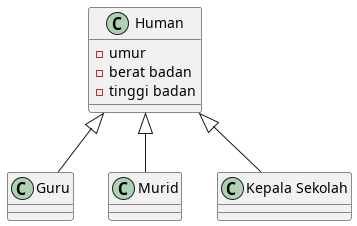
\includegraphics[width=8cm]{inheritance example.png}
        \caption{Contoh dari \textit{inheritance}}
    \end{figure}

    \item \textit{Polymorphism}

    \textit{Child class} adalah sebuah \textit{class} yang akan menuruni semua atribut dan fitur dari \textit{parent class}, tapi apabila dari satu \textit{parent class} memiliki 2 \textit{child class} yang memiliki fitur yang sama tapi cara melakukannya yang berbeda? contoh pisang goreng adalah sebuah makanan, tapi tidak semua makanan adalah pisang goreng, ada perubahan dari cara memasak dan cara penyajian ditiap - tiap makanan, disini konsep \textit{polymorphism} dapat dipakai. Secara definisi \textit{polymorphism} adalah kelakuan dimana \textit{child class} bisa melakukan suatu \textit{task} atau fitur yang sama seperti \textit{parent class} dengan cara yang berbeda\autocite{education-erin-oop-2020}.
\end{enumerate} 

    
\newpage
\subsection*{2.2 \textit{Funtional Programming}}
\addcontentsline{toc}{subsection}{\protect\numberline{}2.2 \textit{Functional Programming}}
\textit{Functional Programming} adalah sebuah konsep, paradigma atau sebuah macam \textit{software development} yang menekankan titik beratnya pada penggunaan \textit{functions}, \textit{Functional Programming} sendiri bukan merupakan sebuah alat yang dapat digunakan tetapi merupakan sesuatu pegangan untuk \textit{developers} sebagai sebuah cara menulis kode\autocite{atencio2016functional}.


Tujuan dari \textit{Functional Programming} adalah membuat sebuah \textit{function} yang lebih kecil yang memiliki sifat dapat digunakkan kembali, lebih dapat diandalkan dan mudah dimengerti, lalu \textit{functions} tersebut maka akan dapat membuat sebuah program yang lebih dapat dimengerti \autocite{atencio2016functional}. \textit{Function} yang dibuat mengikuti \textit{Functional Programming} biasa dibuat dengan melakukan parameterisasi pada \textit{function} supaya dalam menggunakannya dengan menggunakkan parameter kode tersebut dapat digunakkan kembali untuk melakukan hal yang lain. \textit{Functional Programming} memiliki empat konsep dasar, yaitu \textit{Declarative programming}, \textit{Pure functions}, \textit{Referential transparency}, dan \textit{Immutability}\autocite{atencio2016functional}.


\begin{itemize}
    \item \textit{Declarative programming} adalah sebuah pendekatan \textit{programming} dimana sebuah kode untuk melakukan sesuatu akan ditulis menggunakan \textit{expressions} yang mendeskripsikan logika dari suatu program. Berbeda dengan Imperatif atau \textit{Procedural Programming} dimana akan ditulis secara detail bagaimana untuk melakukan sesuatu untuk mencapai hasil yang diinginkan\autocite{atencio2016functional}. 
    \item \textit{Pure functions} adalah \textit{function} yang memiliki dua sifat, yaitu pertama, sebuah pure function hanya dan hanya bergantung pada input yang diberikan dan tidak dengan \textit{state} yang tersembunyi dan/atau external (diluar function tersebut) dan kedua, tidak merubah apapun yang diluar dari \textit{function} tersebut seperti obyek global atau parameter yang di \textit{pass} ke \textit{function} tersebut \autocite{atencio2016functional}. 
    \item \textit{Referential transparency} adalah ketika sebuah \textit{function} menghasilkan hasil yang sama juga diberikan input yang sama \autocite{atencio2016functional}.
    \item \textit{Immutability} adalah dimana dalam \textit{Functional Programming} untuk melestarikan sebuah data supaya \textit{Immutable} tidak bisa diganti setelah di deklarasi. Dalam konsep ini yang perlu diperhatikan adalah object seperti \textit{array} yang dapat berubah konten atau valuenya dalam sebuah function \autocite{atencio2016functional}.  
\end{itemize}

\subsection*{2.3 \textit{Architectural Design}}
\addcontentsline{toc}{subsection}{\protect\numberline{}2.3 \textit{Architectural Design}}

\subsection*{2.4 \textit{Design Pattern}}
\addcontentsline{toc}{subsection}{\protect\numberline{}2.4 \textit{Design Pattern}}

\textit{Design Pattern} secara definisi adalah sesuatu cara komunikasi tiap obyek dan \textit{class} yang dikostumisasi untuk memecahkan masalah desain general didalam konteks tertentu, \textit{design pattern} membantu untuk membuat \textit{object oriented design} yang dapat digunakan secara berulang, dengan cara memberi nama, mengabstraksi, dna mengidentifikasi kunci aspek dari struktur desain tertentu\autocite{design-pattern-2588942}.
\begin{itemize}
    \item \textit{Facade}\\
    \textit{Facade} adalah sesuatu \textit{class} yang memberikan \textit{interface} yang simpel ke sub-sistem yang kompleks, \textit{design pattern} ini dapat digunakan ketika butuh mengintegrasikan sesuatu \textit{library} dengan fitur yang sangat banyak tapi hanya butuh menggunakan beberapa fiturnya saja\autocite{refactoring-guru}. \textit{Singleton} juga memberikan global \textit{access point} ke instansi \textit{class} tersebut, jadi semua \textit{class} dan \textit{object} dapat membaca \textit{value} yang sama dan merubah \textit{value} tersebut secara keseluruhan\autocite{refactoring-guru}.
    \item \textit{Singleton}\\
    \textit{Singleton} digunakan untuk menjamin bahwa suatu \textit{class} hanya memiliki satu \textit{instance}, \textit{design pattern} ini berguna saat ingin mengontrol sebuah \textit{shared resources} seperti \textit{database}\autocite{refactoring-guru}.
    \item \textit{Builder}\\
    \textit{Design pattern} ini dibuat untuk memecahkan masalah ketika ada sebuah \textit{class} yang saat dibuat menjadi sebuah \textit{object} tidak semua atributnya diisi, tanpa harus membuat \textit{contructor} atau \textit{child class} banyak. \textit{Builder} mengekstrasi \textit{building steps} saat membuat suatu \textit{object} dari sebuah \textit{class} dan memindahkannya ke \textit{class} terpisah\autocite{refactoring-guru}.
    \item \textit{Template Method}\\
    \textit{Template method} digunakan untuk mengurangi redudansi ketika ada beberapa fitur dengan langkah penyelesaian sama tapi dengan cara yang berbeda, \textit{template method} dibuat dengan cara memisahkan logika suatu fitur menjadi beberapa langkah dan saat ingin menambahkan fitur baru, bisa langsung membuat \textit{child class} dari \textit{template method} tersebut dan meng-\textit{override} step yang ingin diganti logikanya\autocite{refactoring-guru}.
\end{itemize}

\newpage
\section*{Bab 3. Metode Pelaksanaan}
\addcontentsline{toc}{section}{\protect\numberline{}Bab 3. Metode Pelaksanaan}
\subsection*{3.1 Metode Pelaksanaan}
\addcontentsline{toc}{subsection}{\protect\numberline{}3.1 Metode Pelaksanaan}


Pengumpulan data yang kami lakukan adalah dengan membuat form survei menggunakan \textit{Google Form} untuk mendapatkan pendapat atas pertanyaan-pertanyaan yang kami miliki terkait dengan alasan dari pembuatan aplikasi pada proyek ini. Dari hal mengenai pembelian barang hobi hingga tingkat kesulitan dalam menemukan barang yang cocok. Dari semua jawaban survei yang dikumpulkan tersebutlah, kita dapat memperoleh gambaran dan konfirmasi atas fitur-fitur yang kami butuhkan.


Pertanyaan “Apakah anda takut untuk mengambil hobi baru karena tidak tau mulai dari mana?”, kami ajukan kepada pengisi survei untuk mendapatkan data dan konfirmasi apakah aplikasi dalam proyek kami dibutuhkan, dan dengan hasil jawaban mayoritas diatas 60\% menjawab iya, kami mendapatkan data bahwa terdapat kesulitan memulai hobi karena keraguan titik mulai hobi tersebut.


Selanjutnya dengan “Apakah anda sering menggunakan \textit{e-commerce} untuk browsing dan mencari barang berhubungan dengan hobi anda?” untuk validasi apakah menggunakkan fasilitas online untuk membeli barang hobi itu merupakan metode yang populer. Dengan masukan yang kami dapat diatas 70\% menjawab iya maka kami mendapatkan bahwa fasilitas jual/beli barang hobi di internet itu layak dilakukan.


Untuk pertanyaan “Dalam mencari dan menemukan barang apakah anda terkadang merasa ragu dan harus mencari tahu terlebih dahulu atas barang yang anda lihat apakah untuk pemula/menengah/ahli?” ini adalah untuk mengumpulkan data atas fitur utama yang kami rancang untuk aplikasi ini yaitu fitur filtrasi level kemahiran (\textit{interest level}) dari barang hobi. Dengan respons yang berjawab iya diatas 70\% maka fitur utama kami untuk aplikasi itu layak untuk diimplementasikan.

\subsection*{3.2 Analisis}
\addcontentsline{toc}{subsection}{\protect\numberline{}3.2 Analisis}

\subsubsection*{3.2.1 Analisis perbandingan aplikasi sejenis}
\addcontentsline{toc}{subsubsection}{\protect\numberline{}3.2.1 Analisis perbandingan aplikasi sejenis}
Terdapat dua aplikasi serupa dengan aplikasi didalam proposal proyek ini yang kami jadi obyek oberservasi, yaitu \textit{Reddit} dan \textit{Tokopedia}.

\begin{longtable}{|m{2cm}|p{5cm}|p{5cm}|}
    % \begin{tabular}{| c | c | c |} 
    \hline
    Aplikasi & Positif & Negatif \\ 
    \hline
    Reddit 
    &   + \textit{community} yang sudah besar \newline 
        + System handling \textit{post} dan komen sudah \textit{robust} \newline 
        + Interaksi antara user sudah bagus 
    &   - Bukan marketplace \newline 
        - Tidak cocok untuk memberi rating konkrit kepada barang \newline 
        - Tidak ada gambar atau suatu panel untuk menampilkan informasi item tersebut secara singkat \\ 
    \hline
    Tokopedia
    &   + Proses shipping dan payment sudah berbagai macam \newline  
        + Banyak promo yang bisa didapatkan user  
    &   - Tidak bisa mengelompokkan item berdasarkan hobi \newline 
        - User akan sulit mencari item yang cocok bagi mereka karena ketidakadaannya interest level untuk item tersebut \newline 
        - Tidak ada forum dedikasi diskusi, hanya untuk diskusi barang \\ 
    \hline
\end{longtable}


\subsubsection*{3.2.2 Analisis permasalah}
\addcontentsline{toc}{subsubsection}{\protect\numberline{}3.2.2 Analisis permasalah}
Salah satu pertanyaan adalah "Apakah anda takut untuk mengambil hobi baru karena tidak tau mulai dari mana?" dan dengan responden menjawab 69.2\% iya mereka takut untuk mengambil hobi baru karena alasan yang disebut, beberapa alasan kenapa banyak orang takut untuk mengambil hobi baru adalah, 
\begin{itemize}
    \item mereka tidak tahu apa yang harus dibeli sebagai \textit{beginner};
    \item mereka tidak tahu apa yang mereka beli cocok untuk \textit{interest level} mereka atau tidak;
    \item mereka tidak tahu hal apa saya yang perlu diketahui untuk memasuki hobi tersebut.
\end{itemize}
Dengan 61.5\% menjawab mereka tidak punya waktu untuk mencari tahu informasi tentang hobi tersebut, satu masalah muncul yaitu "bagaimana cara mempercepat proses pemilihan barang untuk pemula hobi".

\subsubsection*{3.2.3 Usulan pemecahan masalah}
\addcontentsline{toc}{subsubsection}{\protect\numberline{}3.2.3 Usulan pemecahan masalah}
Untuk orang yang ingin memulai hobi dan mempunyai banyak waktu untuk mencari informasi tentang hobi tersebut, solusi kami adalah membuat sebuah \textit{marketplace} dengan sebuah \textit{page} yang khusus dibuat untuk para pengguna berdiskusi, berdiskusi tentang sebuah \textit{product} dan ke siapa saja \textit{product} ditujukan.


Untuk orang yang tidak punya waktu untuk melihat semua itu, \textit{project} ini akan menerapkan dua sistem \textit{filter}, \textit{rating} sebuah \textit{product} yang menandakan seberapa berkualitas \textit{product} tersebut dan \textit{rating interest level} dari \textit{product} yang menandakan \textit{product} tersebut itu diarahkan ke siapa. Sistem \textit{interest level rating} ini akan memiliki dua value, \textit{value} pertama adalah \textit{value} yang ditetapkan oleh penjual dan \textit{value} kedua itu yang ditetapkan oleh komunitas, jadi secara tidak langsung jika ada barang yang dengan kedua \textit{rating}nya tidak sama, sipembeli bisa menyimpulkan bahwa penjual ini tidak bisa dipercaya.


\subsection*{3.3 Perancangan}
\addcontentsline{toc}{subsection}{\protect\numberline{}3.3 Perancangan}

\subsubsection*{3.3.1 \textit{Software Design Document}}
\addcontentsline{toc}{subsubsection}{\protect\numberline{}3.3.1 \textit{Software Design Document}}
\begin{enumerate}[label=\alph*. ]
    \item Deskripsi \textit{software}
    
    \textit{Shumishumi} adalah sebuah marketplace dimana user bisa membeli suatu barang sesuai dengan hobi dan setinggi apa \textit{interest level} mereka. Tujuan dari aplikasi ini adalah mempermudah pengguna pembeli untuk mencari barang hobi yang cocok, mempermudah penjual dalam mempromosikan barang-nya kepada pelanggan dengan fitur filter \textit{Interest Level}. 


    \textit{Shumishumi} juga bisa menjadi sarana untuk berdiskusi mengenai topik dan hobi yang diminati, dengan fitur ini kami berharap dapa mempermudah \textit{user} mencari dan memasuki hobi baru.

    \item Fungsi-fungsi \textit{software}

    % sequence diagram

    \item Kebutuhan teknologi

    \begin{enumerate}
        \item \textit{Back end} 

        \textit{Back end} atau bisa disebut juga \textit{developer's end} adalah sebuah layer yang memproses semuanya dibelakang layar dan tempat terjadinya sesuatu yang tidak bisa dilihat oleh \textit{user}\autocite{letsgodojo-frontend-backend}. Analogy yang bisa digunakan adalah saat disebuah restoran ada pelanggan yang memesan sesuatu yang spesifik ke pelayan, ini adalah bagian \textit{front end} dari restoran tersebut, setelah itu pelayan memberikan pesanan tersebut ke koki, yang akan mengambil bahan masak, momotong semua bahan - bahan tersebut, dan memasaknya sesuai resep yang sudah dibuat, koki ini yang merepresentasikan bagian \textit{backend} dari restoran tersebut\autocite{codecademy-backend}. 

        \textit{Back end} terdiri dari dua hal, \textit{servers} yang akan meproses data dan \textit{request} dari sebuah user dan \textit{database} yang akan menyimpan data yang sudah atau yang akan mau diproses\autocite{codecademy-backend}. Dalam proyek ini, kami akan menggunakan \textit{springboot} sebagai \textit{framework} yang digunakan untuk membuat \textit{software back end}-nya dan \textit{\textbf{MySQL}} sebagai database yang digunakan.

        \textit{Springboot} adalah \textit{java back end framework} yang paling populer didunia, \textit{springboot} membuat menulis \textit{software back end} menjadi lebih mudah dan lebih cepat\autocite{spring-framework}, alasan kenapa kami menggunakan \textit{springboot} adalah sebagai berikut:
        \begin{itemize}
            \item \textit{Springboot} mempunyai banyak \textit{plugin} yang dapat di\textit{install};
            \item komunitas \textit{springboot} itu sangat besar;
            \item dan yang terakhir \textit{springboot} memiliki fitur \textit{Inversion of Control} dan \textit{Dependency Injection}.
        \end{itemize}

        \item \textit{Front end}
        
        \textit{Front End} adalah sebuah bagian dari halaman web yang dimana merupakan tempat interaksi pengguna, \textit{Front End} sebagai tempat interaksi pengguna maka merupakan bagian dari sebuah halaman yang sangat sering dilihat oleh pengguna kebalikan dari \textit{Back End}\autocite{codecademy-frontend}.
        
        \textit{Javascript} adalah bahasa pemrograman terkompilasi yang memiliki karakteristik ringan untuk dijalankan, \textit{interpreted} dan juga dengan fitur \textit{first-class functions} dimana \textit{function} dianggap seperti variabel biasa lainnya seperti \textit{string, number,} dan lain-lain. Yang dimana penggunaan \textit{Javascript} paling terkenal dan banyak digunakkan adalah dalam bahasa untuk \textit{Web} atau situs internet\autocite{javascript-mdn}.

        \textit{Typescript} adalah bahasa pemrograman yang dibuat untuk memecahkan beberapa permasalahan yang ada di dalam bahasa \textit{Javascript}, salah satu contohnya adalah dengan \textit{Typescript} penggunaan \textit{Type-annotation} dapat digunakkan untuk memberi tipe dari variabel sehingga permasalahan yang mungkin dapat muncul karena karakteristik \textit{Javascript} yang \textit{loosely typed} dapat diatasi\autocite{fenton2014pro}.

	    \textit{React} adalah sebuah Library untuk bahasa pemrograman \textit{Javascript} (\textit{Typescript} juga bisa) untuk membuat \textit{UI}. Fitur dari \textit{React} adalah \textit{React} menganut \textit{Declarative Programming} dan juga \textit{Functional Programming},\textit{Component Based}, \textit{Hooks} dan \textit{Lifecycle Hooks}\autocite{react-general}. \textit{Hooks} dan \textit{Lifecycle Hooks} adalah sebuah fitur yang diimplementasikan pada \textit{React v16.8} yang memberi alternatif dari menggunakkan \textit{class} untuk komponen\autocite{react-hooks, react-hooks-lifecycle}. 

    \end{enumerate}

\end{enumerate}


\newpage
\subsubsection*{3.3.2 Perancangan Sistem}
\addcontentsline{toc}{subsubsection}{\protect\numberline{}3.3.2 Perancangan Sistem}

\newpage
\addcontentsline{toc}{section}{\protect\numberline{}Referensi}
\printbibliography[title=Referensi]

\end{document}
